\begin{center}
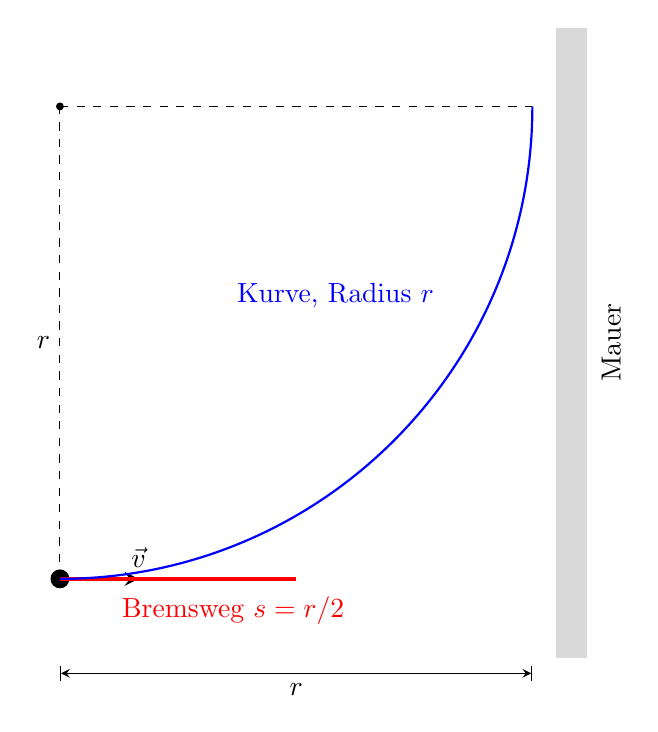
\begin{tikzpicture}[>=stealth]
 \fill[gray!30] (6.3,-1) rectangle (6.7,7);
 \node[rotate=90] at (7.0,3) {Mauer};
 \fill (0,0) circle (0.12);
 \draw[->, very thick] (0,0) -- (1,0) node[above] {$\vec v$};
 \draw[ultra thick, red] (0,0) -- (3,0);
 \node[red, below] at (2.2,-0.1) {Bremsweg $s = r/2$};
 \draw[thick, blue] (0,0) arc[start angle=-90, end angle=0, radius=6];
 \draw[dashed] (0,6) -- (6,6);
 \draw[dashed] (0,0) -- (0,6) node[midway, left] {$r$};
 \fill (0,6) circle (0.05);
 \node[blue] at (3.5,3.6) {Kurve, Radius $r$};
 \draw[|<->|] (0,-1.2) -- (6,-1.2) node[midway, below] {$r$};
\end{tikzpicture}
\end{center}

Beide Manöver werden mit der gleichen maximalen Beschleunigung $a$ gefahren (Haftung der Reifen).

\textbf{Bremsen:} Die Geschwindigkeit nimmt gleichmässig von $v$ auf null ab, die Bremszeit ist $t = v/a$ und die mittlere Geschwindigkeit $v/2$. Der Bremsweg ist
\begin{align}
 s &= \frac{v}{2}\cdot\frac{v}{a} = \frac{v^2}{2a}
\end{align}

\textbf{Ausweichen:} Mit der Radialbeschleunigung $a = v^2/r$ ist der kleinste mögliche Kurvenradius
\begin{align}
 r &= \frac{v^2}{a}
\end{align}
Um einer breiten Mauer auszuweichen, muss das Auto um $\ang{90}$ abbiegen; dabei fährt es noch die Strecke $r$ auf die Mauer zu.

Der Vergleich ergibt
\begin{align}
 \frac{s}{r} &= \frac{v^2/(2a)}{v^2/a} = \result{\frac{1}{2}}
\end{align}
Der Bremsweg ist nur halb so gross wie der Kurvenradius, unabhängig von der Geschwindigkeit. Der Fahrer sollte also \result{bremsen} und geradeaus weiterfahren. (Nur bei einem schmalen Hindernis, an dem man mit einer kleinen seitlichen Verschiebung vorbeikommt, kann Ausweichen günstiger sein.)
